\chapter{Fluorophore Combination Excitation/Emission Spectrograms}

[SECTION UNDER CONSTRUCTION]

Included are spectra views of all multi-stain combinations used. Fluorophores are listed by ascending order of emission peaks. Raw data is available to make each plot indidually if preferable. TBD

Spectrograms Created Using Thermo Fisher Spectra Viewer Application []. Excitation Plots = Dashed Line, Emission Plots = Full Colour Shading.

\begin{figure}[H]
\centering
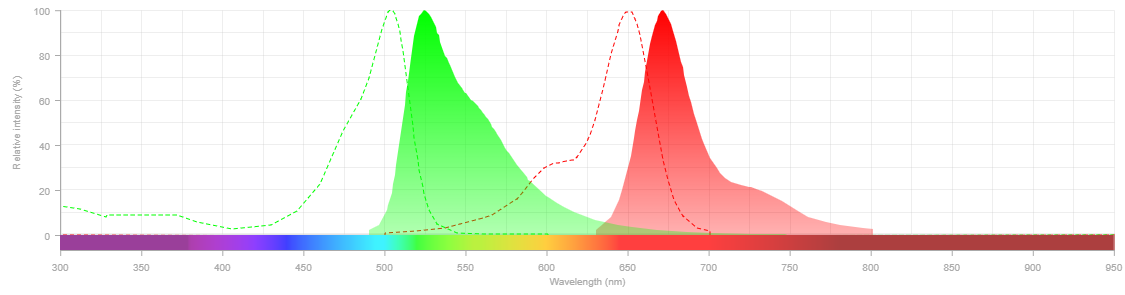
\includegraphics[width=1\linewidth]{Images/spectraviewer.png}
\caption{\textbf{SYTOX Green and Alexa Fluor 647}}
\label{spheroids4.2}
\end{figure}

\begin{figure}[H]
\centering
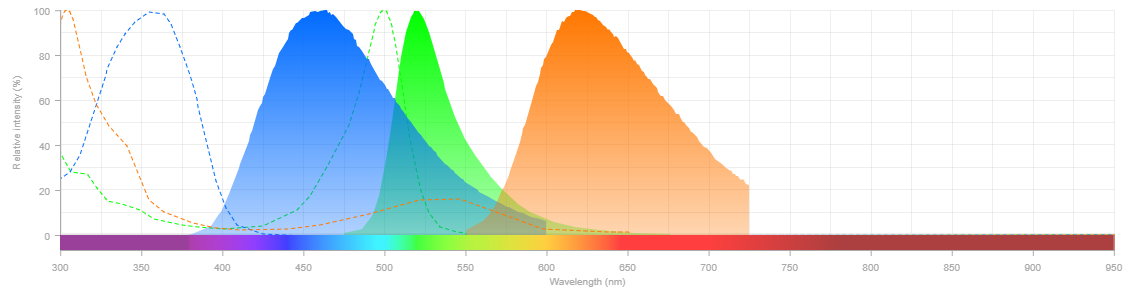
\includegraphics[width=1\linewidth]{Images/spectraviewer (1).png}
\caption{\textbf{DAPI, Alexa Fluor 488, Propidium Iodide}}
\label{spheroids4.2}
\end{figure}

\begin{figure}[H]
\centering
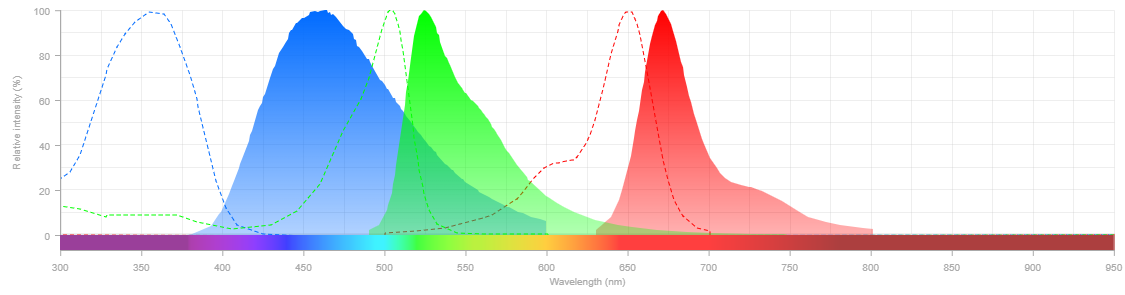
\includegraphics[width=1\linewidth]{Images/spectraviewer (2).png}
\caption{\textbf{DAPI, SYTOX Green, Alexa Fluor 647}}
\label{spheroids4.2}
\end{figure}

\begin{figure}[H]
\centering
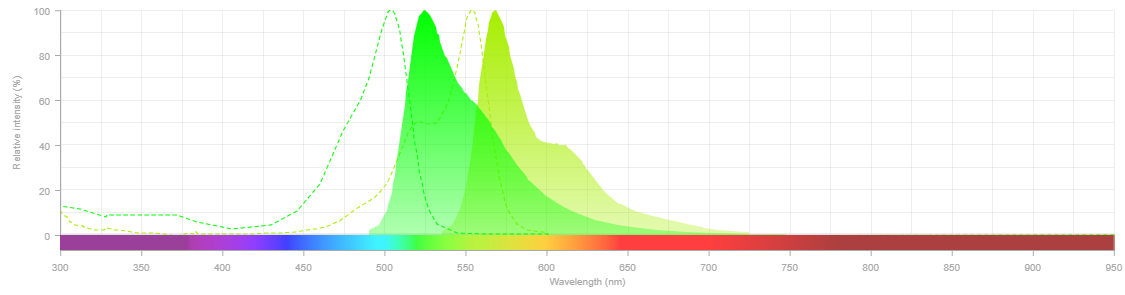
\includegraphics[width=1\linewidth]{Images/spectraviewer (3).png}
\caption{\textbf{Alexa Fluor 555, Propidium Iodide}}
\label{spheroids4.2}
\end{figure}

